\documentclass[10pt,twocolumn,letterpaper]{article}

\usepackage{cvpr}
\usepackage{times}
\usepackage{epsfig}
\usepackage{graphicx}
\usepackage{amsmath}
\usepackage{amssymb}
\usepackage{graphicx}
\graphicspath{{./images/}}
% Include other packages here, before hyperref.

% If you comment hyperref and then uncomment it, you should delete
% egpaper.aux before re-running latex.  (Or just hit 'q' on the first latex
% run, let it finish, and you should be clear).
\usepackage[breaklinks=true,bookmarks=false]{hyperref}

\cvprfinalcopy % *** Uncomment this line for the final submission

\def\cvprPaperID{****} % *** Enter the CVPR Paper ID here
\def\httilde{\mbox{\tt\raisebox{-.5ex}{\symbol{126}}}}

% Pages are numbered in submission mode, and unnumbered in camera-ready
%\ifcvprfinal\pagestyle{empty}\fi
\setcounter{page}{1}
\begin{document}

%%%%%%%%% TITLE
\title{Solving iMet: Fine-grained Multi-label Art Objects Classification with Image-Label Embeddings}

\author{Ekaterina Arkhangelskaia, Olha Sokol\\
Universit{\"a}t des Saarlandes\\
Saarbr{\"u}cken, Germany\\
{\tt\small s8ekarkh,s8olsoko @stud.uni-saarland.de }
}

\maketitle
%\thispagestyle{empty}

%%%%%%%%% ABSTRACT
\begin{abstract}
   People have been collecting art pieces even before our era. Ever since, the amount of art pieces have only been growing. With this increasing growth there is a demand in categorizing and labeling art data. Using manual labor for this purpose can be extremely expensive, therefore an automated solution is needed. Previously, there were some attempts at automated labeling of paintings \cite{Rijks}, however little research have been made in labeling different types of art, like sculpture, ceramics or applied arts. 
   In this project we attempt to perform multi-label classification task on iMet dataset. We utilize label embeddings to improve accuracy of fine-tuned ResNet18 network. Futhermore we use t-SNE algorithm to visualize learned features on artistic data. 

\end{abstract}

%%%%%%%%% BODY TEXT
\section{Introduction}
Art has always been a part of human's life. There are more than 55000 museums in the world, and due to rapid digitilizing of the world a lot of people such as researchers or other scholars would benefit from ability to quickly  navigate among all the data they contain. However, it can be time consuming and inefficient to label all the data by hand. This task motivates us to build end-to-end system to provide automatic labels for sparce and semantically different artistic data. We believe that describing finer-grained attributes from the museum-goer’s understanding, adding fine-grained attributes to aid in the visual understanding of the museum objects will enable the ability to search for visually related objects.

\subsection{Dataset}
%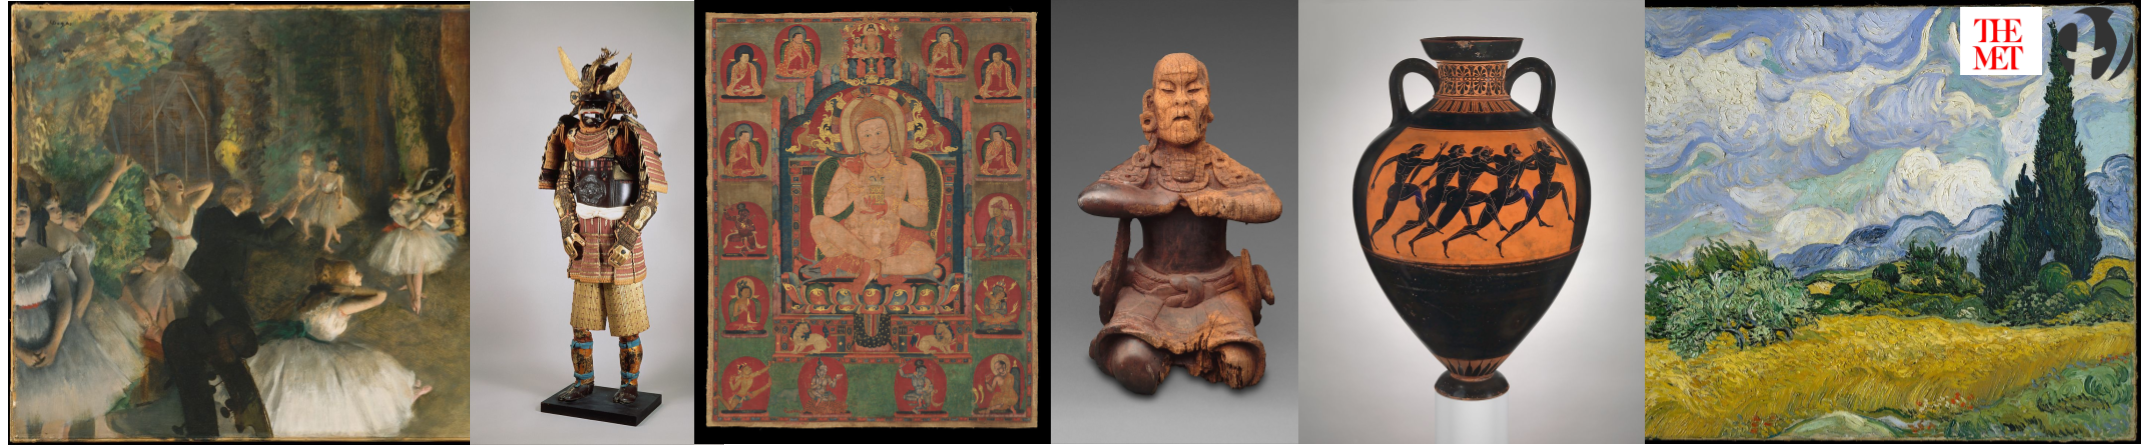
\includegraphics[width=\textwidth]{banner_imet}
\begin{figure}[h!]
\begin{center}
    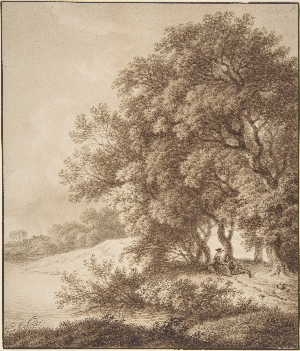
\includegraphics[width=0.25\textwidth]{sample}
\end{center}
  \caption{Sample image from dataset. Culture: central european. Tags: landscapes, lovers, men, trees, woman}
  \label{fig:imet_sample}
\end{figure}
We use iMet dataset from iMet Collection 2019 - FGVC6 challenge \cite{imet}. It is a collection of more than 109k images of different art pieces collected at Metropolitan Museum of Art in New York, also known as The Met.
Each data sample contains one image and at least one attribute label from a label set of 1103 attributes, as can bee seen on Fig \ref{fig:imet_sample}. The dimension of each image is normalized such that the shorter dimension is 300 pixels. Provided annotations are considered somewhat noisy, as they were provided by single worker without verification step. Annotations are devided into 2 categories, culture and tags, tags being related to what is “seen” or what is infered as the object’s “utility.”	

\subsection{Problem statement}
\begin{figure}[h!]
  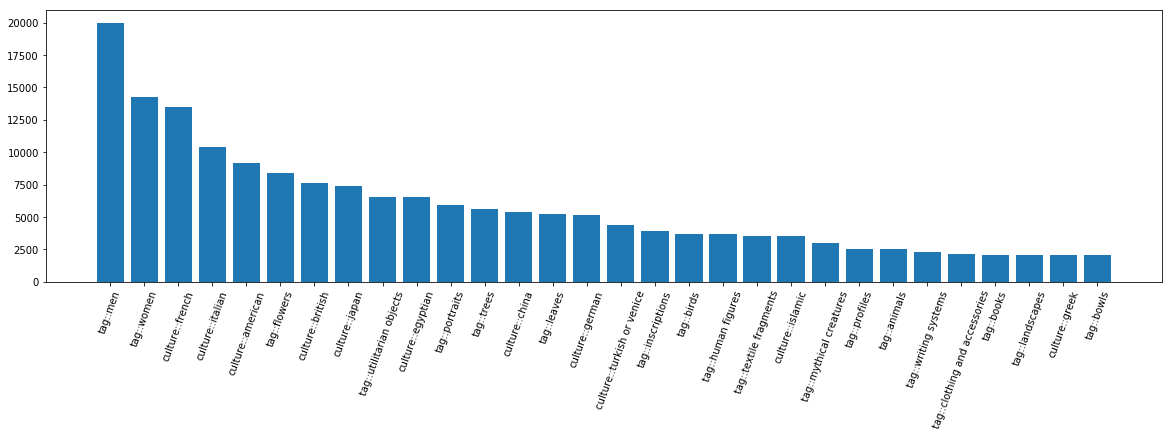
\includegraphics[width=0.5\textwidth]{labels_frequency}
  \caption{Top-30 labels by frequency}
  \label{fig:top30}
\end{figure}


As an input we use single image from iMet dataset, passing it through a neural net we want to receive a set of labels.
As we can see from Fig. \ref{fig:top30}, labels for this dataset are very unbalanced, making training conventional CNNs very challenging. To adress this issue we use labels embeddings to encourage labels close in embedding space to appear together more often.

\subsection{Related work}

There's been a lot of work in classification paintings by author, learning their artistic style  \cite{paint_class}, \cite{rec_style}, \cite{learned_style}, \cite{draw_style}, \cite{la_style}, \cite{la_style_2}, and style transfer \cite{johnson_style_transf}, \cite{huang_style_transf}, \cite{ulyaniv_stylized_img}, \cite{jie_style_transf}. However, little has been made in classification of art pieces that are not paintings. 
T. Balakrishan et al. in \cite{Rijks} tried to classify paintings of Rijksmuseum by their respective authors. To adress imbalance problem they reduces their authors set to include only top 10 artist regarding amount of paintings they produced. Then they used pretrained ResNet-18 and fine-tuned its last layer. However with such architercture they encountered accuracy drop by 0.3\% when increasing number of classes from 10 to 20.


%-------------------------------------------------------------------------

{\small
\bibliographystyle{ieee_fullname}
\bibliography{egbib}
\begin{thebibliography}{9}

\bibitem{Rijks} 
Tara Balakrishan, Sarah Rosston, Emily Tang
\textit{Using CNN to Classify and Understand Artists from the Rijksmuseum}. 
2017.

\bibitem{imet} 

\textit{iMet Collection}. 
 FGVC6, CVPR 2019.

\bibitem{corr_feat}
Wei-Ta Chu, Yi-Ling Wu.
\textit{Deep Correlation Features for Image Style Classification.}
ACM Multimedia 2016.

\bibitem{rec_style}
Sergey Karayev, Aaron Hertzmann, Holger Winnemöller, Aseem Agarwala, Trevor Darrell.
\textit{Recognizing Image Style.}
BMVC 2013.

\bibitem{learned_style}
Vincent Dumoulin, Jonathon Shlens, Manjunath Kudlur.
\textit{A Learned Representation For Artistic Style.}
ICLR 2016.

\bibitem{paint_class}
Wei Ren Tan, Chee Seng Chan, Hernán E. Aguirre, Kiyoshi Tanaka.
\textit{Ceci n'est pas une pipe: A deep convolutional network for fine-art paintings classification.}
IEEE International Conference on Image Processing (ICIP).

\bibitem{draw_style}
Samet Hicsonmez, Nermin Samet, Fadime Sener, Pinar Duygulu.
\textit{DRAW: Deep networks for Recognizing styles of Artists Who illustrate children's books.}
Proceedings of ICMR ’17, June 6–9, 2017, Bucharest, Romania.

\bibitem{la_style}
L. A. Gatys, A. S. Ecker, and M. Bethge.
\textit{A neural algorithm of artistic style.}
arXiv preprint arXiv:1508.06576, 2015.

\bibitem{la_style_2}
L. A. Gatys, A. S. Ecker, and M. Bethge.
\textit{Image style transfer using convolutional neural networks.}
In CVPR, 2016.

\bibitem{johnson_style_transf}
J. Johnson, A. Alahi, and L. Fei-Fei.
\textit{ Perceptual losses for real-time style transfer and super-resolution.}
In ECCV, 2016.

\bibitem{huang_style_transf}
X. Huang and S. J. Belongie.
\textit{Arbitrary style transfer in real-time with adaptive instance normalization.}
In ICCV, 2017.

\bibitem{ulyaniv_stylized_img}
D. Ulyanov, V. Lebedev, A. Vedaldi, and V. S. Lempitsky.
\textit{Texture networks: feed-forward synthesis of textures and stylized images.}
In ICML, 2016.

\bibitem{jie_style_transf}
Jie An, Haoyi Xiong, Jiebo Luo, Jun Huan, Jinwen Ma.
\textit{Fast Universal Style Transfer for Artistic and Photorealistic Rendering}
arXiv preprint arXiv:1907.03118v1, 2019



\end{thebibliography}
}

\end{document}
